\documentclass{article}
\usepackage{fullpage}

%\usepackage{bibentry}
\usepackage{natbib}
% to compile a camera-ready version, add the [final] option, e.g.:
% \usepackage[final]{nips_2017}
\title{Appendix}
\date{}
\author{}
\usepackage[utf8]{inputenc} % allow utf-8 input
\usepackage[T1]{fontenc}    % use 8-bit T1 fonts
\usepackage{hyperref}       % hyperlinks
\usepackage{url}            % simple URL typesetting
\usepackage{booktabs}       % professional-quality tables
\usepackage{amsfonts}       % blackboard math symbols
\usepackage{nicefrac}       % compact symbols for 1/2, etc.
\usepackage{microtype}      % microtypography
\usepackage[utf8]{inputenc} % allow utf-8 input
\usepackage[T1]{fontenc}    % use 8-bit T1 fonts
\usepackage{hyperref}       % hyperlinks
\usepackage{url}            % simple URL typesetting
\usepackage{booktabs}       % professional-quality tables
\usepackage{amsfonts,amsthm}       % blackboard math symbols
\usepackage{nicefrac}       % compact symbols for 1/2, etc.
\usepackage{microtype}      % microtypography
\usepackage{MnSymbol}
\usepackage{color}
\usepackage{graphicx} % more modern
\usepackage{subfigure} 
\usepackage{natbib}
\usepackage{algorithm}
\usepackage{algpseudocode}
\usepackage{lineno}
\usepackage{thmtools,thm-restate}
\usepackage{xr}
\usepackage{xcolor}
\usepackage{tikz}
\colorlet{BLUE}{blue}
\usepackage[normalem]{ulem}

%\linenumbers



\def\A{\mathcal{A}}
\def\ga{\gamma_\mathcal{A}}
\def\Co{C^{\circ}}
\def\Coa{C^{\circ}_{\!\!\mathcal{A}}}
\def\Ca{C_{\!\mathcal{A}}}
\def\go{\gamma^{\circ}}
\def\goa{\gamma^{\circ}_{\A}}
\newcommand{\dt}[2]{\langle#1,#2\rangle}
\def\Olasso{\Omega_{\rm Lasso}} % Lasso norm
\def\Ogl{\Omega_{\rm GL}} % group Lasso norm
\def\Olgl{\Omega_{\rm LGL}} % latent group Lasso norm
\def\Oks{\Omega_{\rm sp,k}} % k-support norm
\def\tr{{\rm tr}}
\newcommand\itgset[1]{[\!\![#1]\!\!]}
\def\RR{\mathbb{R}}
\def\EE{\mathbb{E}}
\newcommand{\tblue}[1]{\textcolor{blue}{#1}}
\newcommand{\tred}[1]{\textcolor{red}{#1}}
\newcommand\TODO[1]{\tblue{TODO: \texttt{#1}}}
%\newcommand\TODO[1]{}
\newcommand\GO[1]{\tred{GO: \texttt{#1}}}
%\newcommand\GOD[1]{\tred{GO: \texttt{\sout{#1}}}}
\newcommand\GOD[1]{}
\newcommand{\GOc}[1]{\todo[backgroundcolor=yellow!50, size=\scriptsize]{#1}}
\newcommand\ra{$\rightarrow$}

\newcommand{\repl}[2]{\textcolor{gray}{\sout{#1}}\: {\textcolor{red}{#2}}}
%\newcommand{\GOcD}[1]{\todo[backgroundcolor=yellow!50, size=\scriptsize]{\sout{#1}}}
\newcommand{\GOcD}[1]{}

\newcommand\OLD[1]{\tblue{#1}}
\newcommand\NEW[1]{\tred{#1}}
\def\st{\text{s.t.}}
\def\supp{\text{supp}}

\def\BIT{\begin{itemize}}
\def\EIT{\end{itemize}}
\def\BET{\begin{enumerate}}
\def\EET{\end{enumerate}}
\def\ra{$\:\rightarrow\:$}
\def\y{\mathbf{y}}
\def\x{\mathbf{x}}
\def\v{\mathbf{v}}
\def\u{\mathbf{u}}
\def\w{\mathbf{w}}
\def\s{\mathbf{s}}
\def\g{\mathbf{g}}
\def\h{\mathbf{h}}
\def\X{\mathbf{X}}
\def\RR{\mathbb{R}}
\def\ei{\varepsilon_i}
\def\ej{\varepsilon_j}
\def\T{\mathcal{T}}
\def\I{\mathcal{I}}
\def\D{\mathbb{R}^p}

\def\op{{\rm op}}
\def\supp{{\rm Supp}}
\def\st{\text{s.t.}}
\newcommand\normop[1]{|||#1|||_{\infty}}
\newcommand\normbop[1]{|\!|\!|#1|\!|\!|_{\infty,2}}
\newcommand\normopop[1]{|\!|\!|#1|\!|\!|_{\rm op,\rm op}}
\newcommand\ve[1]{\varepsilon^{{\scriptscriptstyle#1}}}
\newcommand\sss[1]{{\scriptscriptstyle#1}}
\def\uI{U^{\sss{I}}}
\def\xxi{\zeta}

%\newtheorem{thm}{Theorem}
%\newtheorem{prop}{Proposition}
%\newtheorem{fact}{Fact}
%\newtheorem{lemm}{Lemma}
%\newtheorem{coro}{Corollary}

\newtheorem{lemma}{Lemma}
\newtheorem{lemm}{Lemma}
\newtheorem{cor}{Corollary}
\newtheorem{prop}{Proposition}
\newtheorem{theorem}{Theorem}
\newtheorem{mydef}{Definition}
\newtheorem{ex}{Example}

%AISTATS 2017 experiments
\def \plasso {1000}
\def \nlasso {300}
\def \klasso {8}
\def \mlasso {10}
\def \lambdalasso {5}
\def \rholasso {5}
\def \sigmalasso {0.1}

\def \pwhs{50}
\def \pallwhs{1225}
\def \nwhs {1000}
\def \lambdawhs {5}
\def \sigmawhs {0.1}

\def \lambdacalhous {10^{-3}}

%graph



\begin{document}
\maketitle
\appendix


%\subsection*{Notations}
%In this appendix, we will use two different several norms on matrices, the $\ell_\infty$ norm of the vectorized matrix, also known as the max-norm in the matrix case that we will denote with $\|\cdot\|_{\infty}$.
\section{Abstract lemmas on collections of incoherent subspaces}
The following lemma generalizes a classical upper bound on $|||A^{-1}|||_{\infty}$ discussed in \citet{varga1976diagonal} for diagonally dominant matrices, where $|||\cdot|||_{\infty}$ is the operator $\ell_\infty$ norm (equal to the maximal $\ell_1$-norm of all rows), not to be confused with the 
$\ell_\infty$ norm of the vectorized matrix, also known as the max-norm that we denote with $\|\cdot\|_{\infty}$ throughout the paper.

\begin{lemma}
\label{lem:gbdd}
Let $A=(A_{ij})$ a matrix defining a linear operator from $\RR^{r_1} \times \ldots \times \RR^{r_m}$ to itself, with $A_{ii}=Id_{r_i}$. Consider a collection of norms $\omega_i$ each defined on $\RR^{r_i}$
and define $\omega(x)=\max_i \omega_i(x_i)$. Define the matrix operator norm $|||A|||_{\omega,\omega}=\max_{x:\omega(x)\leq 1} \omega(Ax)$ and consider the quantities:
$\xxi_{ij}=\max_{x_j:\omega_j(x_j) \leq 1} \omega_i(A_{ij}x_j)$.
Then if 
$$\alpha:=1-\max_{i} \sum_{j \neq i} \xxi_{ij}$$ is such that $\alpha >0$, then $A$ is invertible and $|||A^{-1}|||_{\omega,\omega}< \frac{1}{\alpha}$.
\end{lemma}
\begin{proof}
Consider a vector $x$ and assume that $i=\text{arg} \max_{k} \omega_k(x_k)$ then

\begin{eqnarray*}
\alpha \, \omega(x) =\alpha \, \omega_i(x_i) &\leq & \omega_i(x_i) -\sum_{j\neq i} \xxi_{ij}  \, \omega_i(x_i) \leq \omega_i(x_i) -\sum_{j\neq i} \xxi_{ij}  \, \omega_j(x_j)\\
&\leq& \omega_i(Id_{r_i} x_i) -\sum_{j\neq i} \, \omega_i(A_{ij} x_j)
\leq \omega_i(A_{ii} x_i) -\omega_i \big ( \sum_{j\neq i} A_{ij} x_j \big )\\
&\leq&\omega_i \big ( \sum_{j=1}^p A_{ij} x_j \big )
\leq\omega_i (A_{i\cdot}x)=\omega(A x)\\
\end{eqnarray*}

Since this inequality is true for all $x$, it proves that for all $x$, $Ax\neq0$ which entails that $A$ is invertible.
Furthermore,
$$\alpha\leq \inf_{x\neq 0} \frac{\omega(A x)}{\omega(x)}=\inf_{y\neq 0} \frac{\omega(y)}{\omega(A^{-1}y)},$$
given that $y$ is invertible and so $\sup_{y \neq 0}\frac{\omega(A^{-1}y)}{\omega(y)}\leq \frac{1}{\alpha}$ which is the result we want
\end{proof}

\begin{lemma}
\label{lem:two}
In the particular case where there are only two blocks in the previous lemma if $\xxi_{12}\xxi_{21}<1$ then $A$ is invertible and we have $$|||A^{-1}|||_{\omega,\omega} \leq \frac{1+\max(\xxi_{12},\xxi_{21})}{1-\xxi_{12}\xxi_{21}}.$$
\end{lemma}
\begin{proof}
Indeed letting $B:=A_{12}$ so that 
$$A=
\begin{bmatrix}
I & B\\
B^\top & I
\end{bmatrix}
$$
we have that $A$ is invertible if $A^\top A \succ I$, and, in that case
$$A^{-1}=A D \quad \text{with} \quad D:= 
\begin{bmatrix}
(I-BB^\top)^{-1} & 0\\
0 & (I-B^\top B)^{-1}
\end{bmatrix}
$$
Similarly as in the previous proof, letting $\alpha':=1-\xxi_{12} \xxi_{21}$, and using that $\omega_1(BB^\top x_1) \leq \xxi_{12} \omega_2(B^\top x_1) \leq  \xxi_{12} \xxi_{21} \omega_2(x_1),$ 
we have
$$\alpha' \omega_1(x_1) \leq \omega_1(x_1)- \xxi_{12} \xxi_{21} \omega_1(x_1) \leq \omega_1(x_1)- \omega_1(BB^\top x_1) \leq \omega_1 \big ( (I-BB^\top) x_1 \big ).$$
so that if $\alpha'>0$ then $I-BB^\top$ is invertible and so are  $I-B^\top B$,$D$ and $A$. Moreover, we have $|||D|||_{\omega,\omega} \leq \frac{1}{\alpha'}$. Finally, $\omega_1(x_1-Bx_2)\leq \omega_1(x_1)-\omega_1(Bx_2) \leq (1+\xxi_{12}) \omega_1(x_1)$ and symmetrically, $\omega_2(x_2-B^\top x_1) \leq (1+\xxi_{21}) \omega_2(x_2)$, so that $|||A|||_{\omega,\omega} \leq 1+\max(\xxi_{12},\xxi_{21})$ and the result follows using that $|||A^{-1}|||_{\omega,\omega} \leq |||A|||_{\omega,\omega} \, |||D|||_{\omega,\omega}$.
\end{proof}


\begin{cor}
\label{cor:small_x}
Let $\T_i$ a collection of subspaces of $\RR^d$ equipped each with a norm $\Omega_i$. For all $i$, let $\eta_i,\varepsilon_i \in \T_i$ such that
$\Omega_i(\eta_i) \leq \epsilon$. Let $T_i \in \RR^{d \times r_i}$ a matrix whose columns form an orthogonal basis of $\T_i$.  If $\xxi_{ij}(\T_i,\T_j):=\max_{u_j \in \T_j,\: \Omega_j(u_j) \leq 1} \Omega_i(P_i u_j)$, with $P_i:=T_iT_i^\top$ the projector on the subspace $\T_i$. Define $\alpha$ to be the quantity
$$\alpha=1-\max_{i} \sum_{j\neq i} \xxi_{ij}(\T_i,\T_j).$$
Then if, for all $i$, we have that 
$\eta_i=\sum_{j=1}^m P_i\varepsilon_j,$
 and if $\alpha>0$, then the $(\varepsilon_i)_{1 \leq i \leq m}$ are uniquely defined and for all $i,\: \Omega_i(\varepsilon_i) \leq \frac{\epsilon}{\alpha}$.
\end{cor}
\begin{proof}
If $\eta_i, \varepsilon_i \in \T_i$ then there exist unique $b_i$ and $x_i$ in $\RR^{r_i}$ such that $\eta_i=T_i b_i$ and $\varepsilon_i=T_i x_i$.
This entails that the equation $\eta_i=\sum_{j=1}^m P_i\varepsilon_j,$ is equivalent to $b_i=\sum_{j=1}^m T_i^\top T_j x_j$. As a consequence,
if $T:=[T_1,\ldots,T_m]$, let $A:=T^\top T$, then the system of equations relating $\eta:=(\eta_1;\ldots;\eta_m)$ to $x:=(x_1,\ldots,x_m)$ is equivalent to $\eta=A x$.
Moreover if $\omega_i(x_i):=\Omega_i(T_i x_i)$ then the quantities $\xxi_{ij}(\T_i,\T_j)$ and $\alpha$ defined in this corollary match respectively the quantities $\xxi_{ij}$ and $\alpha$ defined from $A$ in Lemma~\ref{lem:gbdd}. By applying the lemma, we thus get that $A$ is invertible and that
$$\max_i\Omega_i(\varepsilon_i)=\max_i \Omega_i(T_i x_i)=\omega(x)=\omega(A^{-1}b)\leq \frac{1}{\alpha} \omega(b)= \frac{1}{\alpha} \max_{i} \Omega_i(T_i b_i)= \frac{1}{\alpha}\max_i\Omega_i(\eta_i) \leq  \frac{\epsilon}{\alpha}.$$
\end{proof}

\begin{cor}
\label{cor:small_x_two}
In the case of two blocks the conclusion of Corollary~\ref{cor:small_x} hold for $\alpha=\frac{1-\xxi_{12}\xxi_{21}}{1+\max(\xxi_{12},\xxi_{21})}$.
\end{cor}
\begin{proof}
This follows from using the bound on $|||A^{-1}|||_{\omega,\omega}$ from Lemma~\ref{lem:two} in the proof of Corollary~\ref{cor:small_x}
\end{proof}


\begin{cor}
\label{cor:main}
Let $\T_i,T_i,P_i,\Omega_i, \xxi_{ij}(\T_i,\T_j)$ and $\alpha$ be defined as in Corollary~\ref{cor:small_x}. Let $(q_i)_{1\leq i \leq m}$ be a given collection of vectors in $\RR^d$ with $q_i \in \T_i$. 
Let $\eta_i=P_i \sum_{j \neq i} q_j$.
Assume that
\BIT
\item the $q_i$ are sufficiently close to orthogonal to the subspaces $\T_j$ for $j \neq i$, so that there exists $\epsilon>0$ with $\max_{i} \Omega_i(\eta_i) \leq \epsilon$.
\item we have $\alpha>0$.
\EIT
Then,  in $\text{span}(\T_1,\ldots,\T_m)$, the set of equations \{$P_i q=q_i, \: \forall i$\} admits a unique solution of the form $q=\sum_{i=1}^m (q_i+\varepsilon_i)$ with $\varepsilon_i$ in $\T_i$ and $\max_i\Omega_i(\varepsilon_i) \leq  \frac{\epsilon}{\alpha}$.
\end{cor}
\begin{proof}
If $q \in \text{span}(\T_1,\ldots,\T_m)$, then $q$ can be written under the form $q=\sum_{i=1}^m (q_i+\varepsilon_i)$ with $\varepsilon_i$ in $\T_i$ and $q$ solves the previous collection of equation if and only if for all $i$
$$q_i=P_i q=q_i +P_i \sum_{j \neq i} q_j+ P_i \sum_{j} \ej.$$
so that if $\eta_i:=-P_i \sum_{j \neq i} q_j$, then $\eta_i$ must satisfy $\eta_i= P_i \sum_{j} \ej$. Furthermore, $\eta$, $\varepsilon$ and the subspace $\T_i$ equipped with the norms $\Omega_i$ together satisfy the conditions of the previous corollary which proves the existence of a solution $q$ of the given form and the announced inequality.
\end{proof}

Note that requiring that $\alpha>0$ in the previous lemma corresponds to a way of quantifying that the subspaces $\T_i$ are \emph{sufficiently incoherent}.

\begin{cor}
\label{car:main_two}
In the case of two blocks, the conclusion of Corollary~\ref{cor:main} holds for $\alpha=\frac{1-\xxi_{12}\xxi_{21}}{1+\max(\xxi_{12},\xxi_{21})}$.
\end{cor}
\begin{proof}
This follows from the same proof as in Corollary~\ref{cor:main} but using Corollary~\ref{cor:small_x_two} instead of Corollary~\ref{cor:small_x}.
\end{proof}

\begin{lemma}
\label{lem:zero_inter}
In the case of two subspaces let $\alpha=\frac{1-\xxi_{12}\xxi_{21}}{1+\max(\xxi_{12},\xxi_{21})}$. Otherwise let $\alpha=1-\max_{i} \sum_{j\neq i} \xxi_{ij}(\T_i,\T_j).$

If $\alpha>0$, then $\forall i, \: \T_i \cap \text{span}\big ( (\T_j)_{j\neq i}\big) =\{0\}$.
\end{lemma}
\begin{proof}
Assume, by contradiction that there exist $(u_i)_{1\leq i\leq m}$, with $u_i \in \T_i$ and
$\sum_{j=1}^m u_j=0$. Then, if $\Omega_i(u_i)=\Omega(u):=\max_j \Omega_j(u_j)$, we have 
$$\Omega(u)=\Omega_i(u_i)=\Omega_i(-P_i u_i)=\Omega_i \big ( \sum_{j \neq i} P_i u_j \big ) \leq \sum_{j \neq _i} \Omega_i(P_i u_j) \leq \sum_{j \neq _i} \xxi_{ij} \Omega_j(u_j) \leq (1-\alpha) \Omega(u).$$ Since $\alpha>0$ this entails $\Omega(u)=0$ and so $u_i=0$ for all $i$. 
\end{proof}




\section{Application to low rank +sparse matrix decompositions}
\subsection{General notations}
We consider several type of subspaces
$$\bar{\T}_I:=\{M \in \RR^{p \times p}\mid  M=M^\top, \: \supp(M)\subset I \times I\},$$
$$\T_I(U):=\{M \in \bar{\T}_I\mid \: M=UX^\top+XU^\top,\: X \in \RR^{\text{rank}(U) \times p} \},$$
Let $\T^c_I(U)$ denote the orthogonal complement\footnote{Note in particular that it is not the orthogonal complement in the entire space.} of $\T_I(U)$ in $\bar{\T}_I$. 
$$\T(U):=\T_{[\![p]\!]}(U)\quad \text{and} \quad \T_s(A)=\{M \in \RR^{p \times p}\mid  \: M=M^\top, \: \supp(M)\subset \supp(A)\}.$$
The projections on the corresponding subspaces are $\mathcal{P}_{\T_s(A)}(M)=M_S$ and $\mathcal{P}_{\T_I(U)}(M)=\mathcal{P}_{U}(M_{II})$ with $$\mathcal{P}_U(M):=M-(I-UU^\top)M(I-UU^\top).$$


\subsection{Convex low rank+ sparse decomposition}
We first show that our assumptions yields results that are different than the one obtained in \citet{chandrasekaran2011rank} and potentially sharper.
\begin{cor}
Consider a matrix $M=A^*+B^*$ as in \citet{chandrasekaran2011rank}. Let 
\begin{eqnarray*}
\mu:=\mu(A^*)&:=&\max \{ \|N\|_{\op} \mid N \in \T(A^*), \|N\|_{\infty} \leq 1\}\\
 \xi:=\xi(B^*)&:=&\max \{ \|N\|_{\infty} \mid N \in \T(B^*), \|N\|_{\op} \leq 1 \}\\
\mu':=\zeta(\T(B^*),\T(A^*))&:=&\max \{ \|\mathcal{P}_{\T(B^*)}(N)\|_{\op} \mid N \in \T(A^*), \|N\|_{\infty} \leq 1\} \\ 
\xi':=\zeta(\T(A^*),\T(B^*))&:=&\max \{ \|\mathcal{P}_{\T(A^*)}(N)\|_{\infty} \mid N \in \T(B^*), \|N\|_{\op} \leq 1 \}\\
\epsilon&:=&\max \big (\|\mathcal{P}_{\T(B^*)}(\gamma \text{sign}(A^*))\|_{\op}, \gamma^{-1}\|UV^\top\|_{\infty} \big ).
\end{eqnarray*}

Let $\alpha:=\frac{1-\mu'\xi'}{1+\max(\gamma \mu',\frac{1}{\gamma} \xi')}$. Then if $\max(\mu,\xi) (1+\frac{\epsilon}{\alpha})<1$, the solution of the optimization problem
$$\min_{A+B=M} \gamma \|A\|_{1}+\|B\|_{\op}$$
has a unique solution which is $(A^*,B^*)$. 
\end{cor}
\begin{proof}
The proof follows the reasoning in \citet{chandrasekaran2011rank} and requires to prove that $\T_s(A^*)\cap \T(B^*)=\{0\}$ and that there exists a subgradient $Q$ of the form $Q=\gamma sign(A^*)+UV^\top+\ve{A}+\ve{B}$, where $B^*=USV^\top$
is the singular value decomposition of $B^*$, and with $\ve{A} \in \T_s(A^*)$,  $\ve{B} \in \T(B^*)$,
such that $\mathcal{P}_{\T_s(A^*)}(Q)=\gamma sign(A^*)$, $\mathcal{P}_{\T(B^*)}(Q)=UV^\top$, $\|\mathcal{P}_{\T_s(A^*)^\bot}(Q)\|_{\infty} <\gamma$ and  $\|\mathcal{P}_{\T(B^*)^\bot}(Q)\|_{\op} <1$. The fact that $\T_s(A^*)\cap \T(B^*)=\{0\}$ follows from applying Lemma~\ref{lem:zero_inter} to the spaces $\T_1=\T_s(A^*)$ and $\T_2=\T(B^*)$ equipped respectively with the norms $\Omega_1=\frac{1}{\gamma}\|\cdot\|_{\infty}$ and $\Omega_2=\|\cdot\|_{\op}$. The fact that and adequate $Q$ exists follows from applying Corollary~\ref{cor:main} with the same subspaces which yields that
$\|\ve{A}\|_{\infty} \leq \gamma \frac{\epsilon}{\alpha}$ and $\|\ve{B}\|_{\op} \leq \frac{\epsilon}{\alpha}$ so that 
$$\|\mathcal{P}_{\T_s(A^*)^\bot}(Q)\|_{\infty}=\|\mathcal{P}_{\T_s(A^*)^\bot}(UV^\top+\ve{B})\|_{\infty}\leq \|UV^\top+\ve{B}\|_{\infty} \leq \gamma \mu \|UV^\top+\ve{B}\|_{\op} \leq \gamma \mu (1+\epsilon/\alpha).$$
$$\|\mathcal{P}_{\T(B^*)^\bot}(Q)\|_{\op}=\|\mathcal{P}_{\T_s(A^*)^\bot}(\gamma sign(A^*)+\ve{A})\|_{\op}\leq \|\gamma sign(A^*)+\ve{A}\|_{\op} \leq \xi \|sign(A^*)+\gamma^{-1}\ve{A}\|_{\infty} \leq  \xi (1+\epsilon/\alpha).$$
\end{proof}

Note that $\mu'\leq \mu$ and $\xi'\leq \xi$ but that $\mu'$ and $\xi'$ are potentially smaller. Also $\epsilon \leq \max(\gamma \mu, \gamma^{-1}\xi)$ but since $\epsilon$ is a bound that holds for the very specific elements $sign(A^*)$ and $UV^\top$ of the tangent spaces $\T(A^*)$ and $\T(B^*)$ and not uniformly over all the tangent space like $\mu', \xi',\mu$ and $\xi'$ it is reasonable to assume that it can be much smaller. 

\subsection*{Low rank with sparse factors + sparse decomposition.}
Let 
\begin{eqnarray*}
\xxi(\T_s(S),\T_J(V))&=&\max \{ {\|M_S\|_\infty} \mid M \in \T_J(V), \: \|M\|_{\op}\leq 1\}\\
\xxi(\T_I(U),\T_s(S))&=&\max \{ {\|\mathcal{P}_{U}(M_{II})\|_{\op}} \mid M \in \T_s(S), \: \|M\|_{\infty}\leq 1\}\\
\xxi(\T_I(U),\T_J(V))&=&\max \{ {\|\mathcal{P}_{U}(M_{II})\|_{\op}} \mid  M \in \T_J(V), \: \|M\|_{\op}\leq 1\}\\
\xi(\T_J(V))&=&\max \{ {\|M\|_\infty} \mid M \in \T_J(V), \: \|M\|_{\op}\leq 1\}\\
\mu_I(\T_s(S))&=&\max \{ {\|M_{II}\|_\op} \mid M \in \T_s(S), \: \|M\|_{\infty}\leq 1\}\\
\end{eqnarray*}

\begin{theorem}
\label{theo:two}
If $M^*=S^*-L^*$ with $L^*=\sum_{I \in \mathcal{I}} L^{\sss{I}}$, $\supp(L^{\sss{I}}) \subset I \times I$ for $\I \subset \mathcal{G}^p_k$ %(where $\mathcal{G}^p_k$ is the collection of all subsets of size $k$ of $[\![p]\!]$) 
and $L^{\sss{I}}=U^{\sss{I}} D^{\sss{I}} {U^{\sss{I}}}^\top$ the eigenvalue decomposition of $L^{\sss{I}}$.
Let $\mu'_I=\xxi(\T_I(U),\T_s(S))$, $\xi'_I :=\xxi(\T_s(S),\T_I(U))$, $\mu_I:=\mu_I(\T_s(S))$, $\xi_I:=\xi(\T_I(U))$, 
$$\alpha_I:=\frac{1-\mu'_I\xi'_I}{1+\max(\gamma \mu'_I,\frac{1}{\gamma} \xi'_I)} \qquad \text{and} \qquad \epsilon_I :=\max \big (\|\mathcal{P}_{\T_I(\uI)}(\gamma \text{sign}(S^*))\|_{\op}, \gamma^{-1}\|\uI {\uI}^\top\|_{\infty} \big ).$$

Assume that for all $(I,I') \in \I \times \I, I \cap I'=\varnothing$. If $$\displaystyle\max_{I \in \I} \max(\mu_I,\xi_I) (1+\frac{\epsilon_I}{\alpha_I})<1, \quad \displaystyle \max_{J \in \mathcal{G}^p_k} \lambda_{\max}^+\big (S^*_{\bar{I}^c \cap (J \times J)} \big ) <1$$ %\quad  
%\text{and}  \quad \max_{J \in \mathcal{G}^p_k, J \neq I}\lambda_{\max}^+(\uI_J{\uI_J}^\top)<1,$$ 
with $\displaystyle \bar{I}=\bigcup_{I \in \I} I \times I$,
then the solution of the optimization problem $$\displaystyle \min \gamma \|S\|_1+\Omega_{k,\succeq}(L) \quad \text{\st} \quad M=S+L$$
 the decomposition given by $\big (S^*,(D^{\sss{I}} \big)_{I \in \I},(\uI)_{I \in \I} \big )$ as a solution.
\end{theorem}
\begin{proof}
We follow the general proof scheme of \citet{chandrasekaran2011rank}. The optimization problem admits the unique announced solution if it satisfies first order gradient condition in the sense that there exists a subgradient $Q \in \RR^{p \times p}$ that satisfies the following conditions
\BET
\item[(i)] for all any $M^\sss{s} \in \T_s(S^*)$ and $(M^{\sss{I}})_{I \in \I}$ with $M^{\sss{I}} \in \T_I(\uI)$, $M^\sss{s}+\sum_{I \in \I} M^{\sss{I}}=0 \: \Rightarrow \: (M^{\sss{I}}=0, \:I \in \I)$.
\item[(ii)] for all $I \in \I,\:\mathcal{P}_{\T_I(\uI)}(Q)=\uI{\uI}^\top$
\item[(iii)] $\mathcal{P}_{\T_s(S^*)}(Q)=\gamma sign(S^*)$
\item[(iv)] for all $I \in \I,\:\lambda_{\max}^+\big (\mathcal(P)_{\T_I^c(\uI)}(Q) \big )<1$
\item[(v)] $\|Q_{S^c}\|_{\infty}<\gamma$
\item[(vi)] for all $J \in \mathcal{G}^p_k \backslash \I, \: \lambda_{\max}^+(Q_{JJ})\leq 1$
\EET
We now prove the different statements. As a consequence of the assumption that $I \cap I'=\varnothing, (I,I') \in \I \times \I,$ the space of symmetric squared matrices can be written as the direct sum of the spaces $(\bar{\T}_I)_{I \in \I}$ and of the space $\T^c:=\{M \in \RR^{p \times p} \mid  M=M^\top, \: M_{\bar{I}}=0\}$. Which entails that part of the properties to prove can be shown independently on the elements of the direct sum, namely the four first properties. 
\BET
\item[(i)] Since $I \cap I'=\varnothing,\: I\neq I'$, we can have $M^\sss{s}+\sum_{I \in \I} M^{\sss{I}}=0$ if and only if $M^\sss{s}_{II}+ M^{\sss{I}}_{II}=0$ for all $I$ and $M^\sss{s}_{\bar{I}}=0$. But if $M^\sss{s}_{II}+ M^{\sss{I}}_{II}=0$ using the argument of \citet{chandrasekaran2011rank} or Lemma~\ref{lem:zero_inter} for two subspaces, we have that $M^\sss{s}_{II}= M^{\sss{I}}_{II}=0$ which shows the result.
\item[(ii)], (iii), (iv) and (v) The existence and the uniqueness of a $Q$ follow from the application of Theorem~\ref{theo:two} to each of the subspaces $(\T_I)_{I \in\I}$ and $\T^c$ separately. The theorem also proves directly that (iii),(iv) and (v) hold.
\item[(iv)] For any $J$ such that $(J \times J) \cap \bar{I}=\varnothing,$ the fact that $\lambda_{\max}^+(Q_{JJ})<1$ follows directly from the fact that then $Q_{JJ}=S^*_{JJ}$ and that $\lambda_{\max}^+(S^*_{(J \times J) \cap \bar{I}^c})<1$.
If $(J \times J) \cap \bar{I} \neq \varnothing$ then let $\mathcal{I}_{J}$ be the collection of sets in $\I$ such that $J$ and $I$ intersect. Note that since these elements $I$ are disjoint $\bar{\T}_J$ is the direct sum of the $(\bar{\T}_{J\cap I})_{I \in \I_{J}}$ and of their orthogonal complement in $\bar{\T}_J$.
As a consequence
$$\lambda_{\max}^+(Q_{JJ}) \leq \Big ( \lambda_{\max}^+(Q_{(J \times J) \cap \bar{I}^c}) \Big ) \vee \max_{I \in \I_{J}} \lambda_{\max}^+(Q_{(J\cap I) \times (J \cap I)}).$$
But $\lambda_{\max}^+(Q_{(J \times J) \cap \bar{I}^c}) <1$ as before and 
we need to show that $\lambda_{\max}^+(Q_{(J\cap I) \times (J \cap I)}) \leq 1.$
%Since $Q_{(J\cap I) \times (J \cap I)=\uI_J\uI_J$
\EET
\end{proof}

Consider a set of indices $J$, which will be fixed throughout this section\footnote{Although most of the variables defined in this section depend on $J$, we do not make this dependence explicit to lighten notations.}.

Denote $u_i:=u_{I_i}$, $\check{u}_i=u^{I_i}_J$ and $v_i:=\frac{\check{u}_i}{\|\check{u}_i\|}$. Let $\kappa:=|\{i \mid I_i \cap J \neq \varnothing\}|.$ Let $k_i:=|I_i \cap J|$. Since, we assume that all the entries of $u_i$ are in the interval $[\underline{\tau}, \overline{\tau}]$, note that we have $k_i \underline{\tau} k_i \leq (\check{u}_i^\top v_i)^2 \leq k_i \overline{\tau}$.

Let $V_i^c \in \RR^{p \times k-1}$ be such that $[v_i, V_i^c]$ forms an orthonormal basis of $\text{span}(e_j)_{j \in J \cap I_i}$. 

Let $V:=[v_1,\ldots,v_\kappa] \in \RR^{k \times \kappa}$ and $V^c:=[V_1^c,\ldots, V^c_\kappa] \in \RR^{k \times   (k-1) \kappa}$. 

By construction, $[V,V^c]$ is an orthonormal basis of $\text{span}(e_j)_{j \in J}$.
Then we have $Q_{JJ}=[V,V^c] \check{Q}_{JJ} [V,V^c]^\top$ with

$$\check{Q}_{JJ}=
\begin{bmatrix}
V^\top Q V & V^\top Q V^c\\
{V^c}^\top Q V & {V^c}^\top Q V^c\\
\end{bmatrix}
$$

We have $[V^\top Q V]_{ii}=v_i^\top Q v_i=v_i^\top [u_i u_i^\top+R_i] v_i$
with $R_i=\mathcal{P}_{\mathcal{T}^{\bot}_{I_i}(u_i)}=(I-u_i u_i^\top)\, Q_{I_iI_i}\,  (I-u_i u_i^\top).$

We have on the one hand, $v_i^\top u_i u_i^\top v_i=(\check{u}_i^\top v_i)^2 \leq k_i \overline{\tau}^2$. On the other, if $\check{v}_i:=(I-u_iu_i^\top) v_i$ then 
$$v_i^\top R_i v_i=(u_i u_i^\top v_i +\check{v}_i)^\top R_i (u_i u_i^\top v_i +\check{v}_i)=\check{v}_i^\top R_i \, \check{v}_i \leq \|R_i\|_{\op} \, \|\check{v}_i\|^2_2 \leq (1-k_i\underline{\tau}^2) \|R_i\|_{\op}$$

So finally, since $\|R_i\|_{\op} \leq \|\gamma sign(S_{I_iI_i})+\varepsilon^{s_i}\|_{\op} \leq \xi_i (1+\frac{\epsilon}{\alpha}),$ we have 
$$v_i^\top Q v_i \leq k_i \overline{\tau}^2+(1-k_i\underline{\tau}^2) \xi_i (1+\epsilon/\alpha).$$
 
 
Then for $[V Q V^c]$, the fact that $v_i$ is proportional to the projection of $u_i$ on ${\rm span}(e_j)_{j \in J}$, we have $u_i^\top V^c=0$ so that

$$\|v_i^\top Q V_i^c\|_{\op}=\|v_i^\top R_i V_i^c\|_{\op} \leq \|v_i^\top R_i\|_{2}.$$
 
\begin{lemma}
If $u$ is a vector such that $\|u\|_2=1$, then we have
 $\|u^\top Z\|_{2} \leq \|\mathcal{P}_{\mathcal{T}(u)}\|_{\op}  \leq 2\, \|u^\top Z\|_{2}.$
\end{lemma}
\begin{proof}
We use the following key identity
 
 $$\mathcal{P}_{\mathcal{T}(u)} u=(uu^\top Z + Z uu^\top - u u^\top Z u u^\top) u =Zu$$

$$\|\mathcal{P}_{\mathcal{T}(u)}\|_{\op} \geq \|u^\top \mathcal{P}_{\mathcal{T}(u)}\|_{2} \geq \|u^\top (uu^\top Z + Z uu^\top - u u^\top Z u u^\top) \|_{2}=\|u^\top Z\|_{2}
$$
\begin{eqnarray*}
\|\mathcal{P}_{\mathcal{T}(u)}\|_{\op}:=\|uu^\top Z + Z uu^\top - u u^\top Z u u^\top\|_{\op}  
& \leq & \, \|uu^\top Z\|_{\op} + \|Z uu^\top - u u^\top Z u u^\top\|_{\op}\\
& \leq &  \, \|u^\top Z\|_{2} + \|Z uu^\top - u^\top Z u u^\top\|_{2}\\
& \leq &  \,\|u^\top Z\|_{2} + \sqrt{u^\top Z^2 u - u^\top Z u }\\
& \leq & 2 \, \|u^\top Z\|_{2}
\end{eqnarray*}
\end{proof}

To summarize

$$\check{v}_i^\top Q \check{v}_j=v_i^\top u_i u_i^\top [Q_{S}]_{I_i I_j} u_j u_j^\top v_j$$

%$u_i^\top Z u_j$

$$|u_i^\top Z u_j| = |u_i \mathcal{P}_{\mathcal{T}(u_j)}(Z) u_j^\top|=|u_i \mathcal{P}_{\mathcal{T}(u_i)} \circ \mathcal{P}_{\mathcal{T}(u_j)}(Z) u_j^\top| \leq \|\mathcal{P}_{\mathcal{T}(u_i)} \circ \mathcal{P}_{\mathcal{T}(u_j)}(Z)\|_{\op} \leq \xi_{ij} \|\mathcal{P}_{\mathcal{T}(u_j)}(Z)\|_{\op} \leq \zeta_{ij} \zeta_{js}.$$

We can use similar ideas to bound:
\begin{itemize}
\item $\check{v}_i^\top Q \check{v}_j$ 
\item $v_i^\top Q v_j$
\item $\|v_i^\top Q V_j^c\|_2$
\end{itemize}

%$$
%\begin{bmatrix}
%v_1^\top u_1 u_1 ^\top v_1 & v_1^\top Q_S^\top v_2 & \ldots & v_1^\top Q_S^\top v_\kappa v_1^\top Q_S^\top V_1 & \ldots & v_1^\top Q_S^\top V_\kappa\\
%v_2^\top Q_S^\top v_1 & v_2^\top u_2 u_2 ^\top v_2 & \ldots & v_2^\top Q_S^\top v_\kappa v_2^\top Q_S^\top V_1 & \ldots &  v_2^\top Q_S^\top V_\kappa\\
%\vdots & \ddots & \ldots & & \\
%v_\kappa^\top u_1 u_1 ^\top v_1 & \ldots v_\kappa^\top Q_S^\top v_2 & \ldots v_{\kappa}^\top u_\kappa u_\kappa ^\top v_\kappa& v_\kappa^\top Q_S^\top V_1 & \ldots & v_\kappa^\top Q_S^\top V_\kappa\\
%\end{bmatrix}
%$$


%Assume that for all $(I,J) \in \I \times \I$
%
%
%
%If $M^*=S^*-L^*$ with $L^*=\sum_{I \in \mathcal{I}} L^{\sss{I}}$, $\supp(L^{\sss{I}}) \subset I \times I$ and $L^{\sss{I}}=U^{\sss{I}} D^{\sss{I}} {U^{\sss{I}}}^\top$ the eigenvalue decomposition of $L^{\sss{I}}$.
%
%Assumptions:
%
%Let $\tilde{Q}:=\sum_{I \in \mathcal{I}} U^{\sss{I}} {U^{\sss{I}}}^\top$, $m_{ij}=|\{I \in \mathcal{I} \mid I \ni (i,j) \}|$ and 
%$m^*=\max_{(i,j) \in [\![p]\!]^2} m_{ij}$, $\xi=\max_{I \in \mathcal{I}} \xi(\T_I(U^{\sss{I}}))$, $\mu=\max_{I \in \I} \mu_I(\T_s(S))$.
%
%Let 
%$$\sigma:=\min_{I \in \I}\lambda_{\min} \big (\mathcal{P}_{\T(\uI)^\bot} (\tilde{Q}+\gamma sign(S^*)) \big ) \quad {and} \quad \lambda=\max_{I \in \I}\lambda_{\max}^+ \big (\mathcal{P}_{\T(\uI)^\bot} (\tilde{Q}+\gamma sign(S^*)) \big ) $$
%\BIT
%\item[($*$)] $\|\tilde{Q}_{S^c}\|_{\infty} < \gamma(1-\xi m^*  \frac{\alpha}{\epsilon})$
%\item[($**$)] $\sigma> (\mu \gamma^{-1}+(m^*-1)) \frac{\epsilon}{\alpha}$.
%\item[($***$)] $\lambda< 1-\mu \gamma^{-1}\frac{\epsilon}{\alpha}$.
%\item[($****$)] $\gamma \max_{J \in \mathcal{G}^p_k} \lambda^+_{\max}(sign(S_{JJ})) < 1$.
%
% 
% \begin{eqnarray*}
% \max_{I \in \I}\lambda_{\max}^+\Big (\mathcal{P}_{\T(\uI)^\bot} \big (\tilde{Q}_{II}-\uI {\uI}^{\top}\!\!+\gamma sign(S^*_{II})\big )  \Big )&<&1-(m^*-1+\mu \gamma) \frac{\epsilon}{\alpha}\\ 
%\max_{J \in \mathcal{G}^p_k}\lambda_{\max}^+\Big (\tilde{Q}_{JJ}+\gamma sign(S^*_{JJ}))\Big )&<&1-(m^*-1+\mu \gamma) \frac{\epsilon}{\alpha}
%\end{eqnarray*}
%\EIT
%
%
%We have $\|Q_{S^c}\|_{\infty} < \gamma$ since
%
%$$\gamma^{-1} \|Q_{S^c}\|_{\infty}=\gamma^{-1} \|\tilde{Q}_{S^c}+\sum_{I \in \I} \ve{I}_{S^c}\|_{\infty} \leq \|\tilde{Q}_{S^c}\|_{\infty} + \sum_{I \in \I} \|\ve{I}_{S^c}\|_{\infty} \leq \|\tilde{Q}_{S^c}\|_{\infty}+m^* \gamma  \, \xi \frac{\epsilon}{\alpha}.$$
%
%To show that $\lambda_{\max}^+(Q_{JJ})\leq 1$ for all $J$, we first show that under ($**$) we necessarily have $\ve{I}\prec 0$ for all $I \in \I$. 
%
%Indeed,
%$$-\ve{I}=\mathcal{P}_{\T_I(\uI)} \big ( \tilde{Q}-\uI {\uI}^\top + \gamma sign(S^I)+ \ve{S}+\sum_{J \in \I, \, J \neq I} \ve{J}\big ).$$
%So that 
%$$\lambda_{\min}(-\ve{I}) \geq \sigma-\|\ve{S}_I\|_{\op}-\!\!\!\sum_{J \in \I, \, J \neq I} \|\ve{J}_I\|_{\op} \geq \sigma - (\mu \gamma^{-1}+(m^*-1)) \frac{\epsilon}{\alpha}>0,$$
%by Assumption ($**$).
%
%On the subspace $\T_I(\uI)^{\bot}$, we have
%\begin{eqnarray*}
%\lambda^+_{\max}\Big ( \mathcal{P}_{\T_I(\uI)^{\bot}} \big (\tilde{Q}+ \gamma sign(S_{II})+ \ve{S}_{II}+\sum_{J \in \I, \, J \neq I} \ve{J} \big ) \Big) &\leq & \lambda^+_{\max}( \tilde{Q}+\gamma sign(S_{II})+ \ve{S}_{II})\\
% &\leq& \lambda^+_{\max}( \tilde{Q}+\gamma sign(S_{II})) + \mu \gamma \frac{\epsilon}{\alpha} \\
% &<& 1
%\end{eqnarray*}
%where the first inequality follows from the fact that $\ve{I}\prec 0$ and the last one from Assumption ($***$).
%
%We now consider bounding $\lambda_{\max}^+(Q_{JJ})$ for $J \notin \I$.
%First assume the case where $J \cap I=\varnothing$ for all $I \in \I$.
%In that case we have $Q_{JJ}=\gamma sign(S_{JJ})$ and the result follows directly from Assumption ($****$).


%$$\sigma-\|\ve{S}_I\|_{\op}-\!\!\!\sum_{J \in \I, \, J \neq I} \|\ve{J}_I\|_{\op} \geq \sigma - (\mu \gamma^{-1}+(m^*-1)) \frac{\epsilon}{\alpha}>0,$$

\section{A theory of unmixing by gauge minimization}

A common problem in the signal processing literature which is also highly relevant in the machine learning and statistics communities is the decomposition or unmixing problem: given $y=\sum_{i=1}^{m}x_{i}^*$ with all $x_{i}^*$ belonging to a vector space $\mathcal{D}$ and some prior information on the characteristics or structure of the $x_{i}^*$, under what conditions are they identifiable unambiguously? \GO{Need to see if there are some references that are appropriate here.}

In particular, we are interested by the case where each $x_{i}^*$ is ``simple'' for a given measure of complexity which is a norm or gauge $\omega_i$, and which encourages properties such as sparsity, low rankness and, more generally, the fact that $x_{i}^*$ belongs to a union of subspaces or submanifolds associated with the gauge. The most emblematic example of this type of decomposition in the recent literature is probably the sparse + low rank matrix decomposition problem studied in \citet{chandrasekaran2011rank}. \GO{TODO: We need to say that in fact there are other of instances of decomposition problem of this form in the literature like robust PCA (papers of Cand\`{e}s + papers of Caramanis), union of subspace models (see Rene Vidals's papers with Elhamifar). We should also say that latent group Lasso formulation are naturally of this form (including the ``dirty statistical models'' of Ali Jalali) and that there are tensor decomposition formulations like with the latent trace norm of Tomioka and Kishan Wimalawarne (see ref in the tex file).
%Wimalawarne, K., Sugiyama, M., & Tomioka, R.  Multitask learning meets tensor factorization: Task imputation via convex optimization.  In Z. Ghahramani, M. Welling, C. Cortes, N. D. Lawrence, and K. Q. Weinberger (Eds.), Advances in Neural Information Processing Systems 27, pp.2825-2833, 2014. (Presented at Neural Information Processing Systems (NIPS2014), Montreal, Quebec, Canada, Dec. 8-11, 2014).
To the best of our knowledge, recovery guarantees have only been studied in the case for the case of unmixing two components and not three or more. 
}

The motivation for considering gauges is that is to common to consider underlying structures that are combinatorial, like sparsity and would lead to untractable formulations for the characterization of $x_i^*$. More precisely, in a number of settings, is it natural to assume that $x_i^*$ is a combination of a small number of elements of the ambient vector space, called \emph{atoms}, and picked in a collection $\mathcal{A}_i$, and a gauge naturally associated with this type of structure
is the atomic gauge \GO{cite paper of Chandrasekaran on atomic gauges} associated with $\mathcal{A}_i$.

We formulate the problem of recovering the components $x_i^*$ as a that of finding a minimal complexity decomposition, as follows
\begin{equation}
\label{eq:gen_opt}
\min_{x_{1}, \ldots, x_{m} \in \,\D} \quad \sum_{i=1}^{m} \gamma_{i}\, \omega_{i}(x_{i})
\qquad \text{s.t.} \quad y=\sum_{i=1}^{m}x_{i},
\end{equation}
where $\gamma_{i}>0$ are  user-defined regularization parameters. \GO{Is it actually useful to have $\gamma_i$ here? Can't they be implicitly encoded in $\omega_i$?}


The question that we investigate in the next section is under what conditions on $x_i^*$ and $\omega_i$ are the components $x_i^*$ the unique solution of problem~\eqref{eq:gen_opt}.

\subsection{Subspace associated with a gauge at a point}

If the gauges $\omega_i$ were simply indicators of linear subspaces $\T_i$ of $\RR^p$, it would be sufficient for problem \eqref{eq:gen_opt} to have a unique solution that the collection of subspaces $\T_i$ are linearly independent in the sense that for any $i$, $\T_i \cap \text{span}(\T_j)_{j \neq i}=\{0\}$. 

As will show, under some appropriate hypotheses, a gauge $\omega$ naturally associates to an element $x \in \D$ a subspace $\T_x$ containing $x$ and which, as we will discuss in Section ~\ref{} play essentially the same role as the spaces $\T_i$ in the previous discussion. In particular cases, this subspace seem to coincide with the notion of tangent space used in \citet{chandrasekaran2011rank} and as a way to formalize the concept of \emph{decomposable norms} introduced in \citet{negahban2012unified}. Concepts related to \emph{decomposable norms} with stronger ground in convex analysis that were then proposed in \citet{candes2013simple} and extended to gauges in \citet{vaiter2015model} \citep[see also][]{fadili2013stable,vaiter2015low}.

Following closely some of the ideas of~\citet{vaiter2015model}, we introduce a simple definition leading to a construction of the space $\T_x$. 

\begin{mydef}
We say that the gauge $\omega$ has an \emph{orthogonally decomposable subgradient} at $x \in \RR^p$ if the projection of the origin $0$ on the affine span of $\partial \omega(x)$ is in $\partial \omega(x)$.
\end{mydef}
\GO{I removed he relative interior condition. TODO for G: double check why \citet{vaiter2015model} impose that condition. This would be a problem when working with gauges defined on cones that are direct sums of a points and a cone because then $q_x$ is not in the relative interior of the cone...}


This terminology is motivated by the following characterization by~\citet{vaiter2015model}:

\begin{prop}
\label{prop:ods}
If $\omega$ has an o.d.s.\ at $x$ then, denoting the projection of the origin $0$ on the affine span of $\partial \omega(x)$ by $q_x$, letting 
$Q_x:=\partial \omega(x)-q_x$, and
$\T_x:=\text{span}\big (Q_x\big)^{\bot}$ the subspace orthogonal\,\footnote{If the gauge $\omega$ has a domain (i.e. $\{x \mid \omega(x)< \infty \}$) which is included in a strict subspace $\mathcal{E}$ of $\RR^p$ then $\T_x$ can also be defined as the orthogonal complement of $\text{span}(Q_x)$ in $\mathcal{E}$ and not in $\RR^p$.} to $Q_x$
 then 
\BIT
\item $x, q_x \in \T_x$,
\item $\partial \omega(x)$ decomposes orthogonally on $(\T_x,\T_x^{\bot})$ in the sense that $\partial \omega(x)=\{(q,q') \mid (q,0)=q_x, \: (0,q') \in Q_x\}$ is a cartesian product.
\EIT
In other words, if $\omega_x^{\bot,\circ}$ denotes the gauge of $Q_x$ then we have $\partial \omega(x)=\big \{q \mid P_{\T_x}q=q_x, \:\: \omega_x^{\bot,\circ}\! (q-q_x) \leq 1\big\}.$ 
\end{prop}

Note that $\omega_x^{\bot,\circ}(q')=\omega^{\circ}(q_x+q')+\iota_{\T_x^{\bot}}(q')$.\vspace{2mm}

Natural examples of gauges with o.d.s.\ are provided by \emph{separable}/\emph{decomposable} norms~\citep{negahban2012unified}.

\begin{mydef}
Given a pair of subspaces $\mathcal{M}$ and $\mathcal{T}^{\perp}$ a norm $\omega$ is
\emph{separable} on $(\mathcal{M},\mathcal{T}^{\perp})$ if
$$
\omega(x+y)=\omega(x)+\omega(y) \quad \forall (x,y)\in\mathcal{M}\times\mathcal{T}^{\perp}.
$$
\end{mydef}

In particular if $\omega$ is separable on $(\mathcal{M},\mathcal{M}^{\perp})$ and $x \in \mathcal{M}$ is a point at which the restriction of $\omega$ to $\mathcal{M}$ is differentiable, then $\omega$ has an o.d.s.\ at $x$ with $q_x=\nabla (\omega|_{\mathcal{M}})(x)$ and $Q_x=\partial (\omega|_{\mathcal{M}^{\perp}})(0).$ Note that we must have $\mathcal{M} \subseteq \T_x$. There are many examples of norms separable on a pair $(\mathcal{M},\mathcal{M}^{\perp})$, including the Lasso and the group-Lasso.
The trace norm is also separable but for a pair of spaces $(\mathcal{M},\mathcal{T}^{\perp})$ that are not the orthogonal complement of each other; however, given the form of the subgradient of the trace norm, it is easy to see that it satisfies the o.d.s. property as well.

Note that separability at $x$ alone is not sufficient to obtain an o.d.s.\ property, and vice-versa, the o.d.s.\ property does not imply separability. In particular, it is easy to see that a number of norms that are not separable have the o.d.s.\ property: we can cite among others some OWL norms like SLOPE and more generally the locally decomposable norm considered in \citet{obozinski2016unified}. This mismatch of concepts has led different authors to make assumptions that are hybrid between the o.d.s.\ property above and separability~\citep{candes2013simple,fadili2013stable,vaiter2015model}.

The o.d.s.\ property that we defined, while convenient, is in fact not necessary for the rest of our analysis and could be relaxed, to generalize our results to any (coercive) gauge. What is actually key is the fact that for any $q_x \in \partial \omega(x)$, the subspace $T_x:=\text{span}(q-q_x)^{\bot}$ is the same and that we have $x \in \T_x$, which is true for any gauge. 
The o.d.s.\ assumption could therefore be generalized by replacing the orthogonal projection in the definition by an oblique projection. We do not consider this extension for simplicity, because in general the oblique projection is not defined in a unique way, and because we do not have concrete interesting examples of regularizers where the general case would be needed. 



\GO{Interesting question: can $\T_x$ be interpreted as a tangent space to a manifold associated with the gauge? If so what is this manifold?}

\subsection{Examples of gauge with an orthogonally decomposable subgradient}

\GO{This section needs to be rewritten: we need to revisit the examples below based on the new definition.} 
Natural examples of are the trace norm for inducing low rank structure and $\ell_1$ norm for inducing sparsity \TODO{detail spaces $\mathcal{M}$ and $\mathcal{M}^{\perp}$ ?}.\\

\paragraph{$\|.\|_1$ norm for matrices in $\RR^{p\times p}$: } Let $S$ be any particular subset of indices, then $\|.\|_1$ is decomposable with respect to $\mathcal{A}(S):=\left\lbrace M\in\RR^{p\times p} \enskip | \enskip M_{ij}=0\:\: \text{if} \:\: (i,j) \notin S\right\rbrace$ and $\mathcal{B}(S):=\left\lbrace M\in\RR^{p\times p} \enskip | \enskip M_{ij}=0 \:\: \text{if} \:\: (i,j) \in S\right\rbrace$.

\paragraph{$\|.\|_{tr}$ norm for p.s.d.\ matrices in $\RR^{p\times p}$: } If $M$ is a p.s.d.\ matrix and $M=USU^{\top}$ its eigenvalue decomposition, then $\|.\|_{tr}$ is decomposable with respect to $\mathcal{A}(U):=\left\lbrace USU^{\top} \enskip | D \enskip \text{diagonal}\right\rbrace$ and $\mathcal{B}(U):=\left\lbrace N\in\RR^{p\times p} \enskip | U^{\top}N=0 \enskip \text{and} \enskip N \succeq 0\right\rbrace$.\\


\GO{It could be nice to discuss what happens in general for an atomic norm: while it might be difficult to say exactly when it has the o.d.s.\ property, I have the impression that we have something like $Q_x \subset \{q \mid \langle q, a_i \rangle =0 \}$ so that $\T_x =\text{span} \big (\{a \in \mathcal{A} \mid \langle a, a_i \rangle =0\} \big )^\bot$ in that case. Or is just $\subset$? To think about...}

\subsection{Identifiability conditions for unmixing by gauge minimization}

%Concretely, we focus on studying the exact recovery of $(x_{1}^*,x_{2}^*,..,x_{m}^*)$ from the optimization problem 
%\begin{align}
%\label{eq:gen_opt}
%\min_{x_{1}, \ldots, x_{m} \in \,\D} &\quad \sum_{i=1}^{m} \gamma_{i}\, \omega_{i}(x_{i})\\
%&\text{s.t.} \quad y=\sum_{i=1}^{m}x_{i}, \nonumber
%\end{align}
%where $\gamma_{i}>0$ are  user-defined regularization parameters. 


Without any appropriate assumptions, problem (\ref{eq:gen_opt}) is in general not well posed and even if the solution is unique there is no guarantee that the obtained decomposition yields the $x_i^*$.

However, under some incoherence conditions on tangent spaces we prove that the decomposition is exactly recovered. Proposition \ref{prop:genunicity} states existence and uniqueness \GO{[uniqueness is better English that unicity]} of the solution of (\ref{eq:gen_opt}) and theorem \ref{theo:gentwo} states simple conditions that guarantee exact decomposition for problem  (\ref{eq:gen_opt}). %However, under some incoherence conditions on tangent spaces we prove that the decomposition is exactly recovered. In order to characterize incoherence conditions, we will remind the concepts of incoherence and tangent spaces.  We will extend the notion of incoherence to collections of subspaces.

\NEW{For all $i$, we consider the subgradient of the gauge $\omega_i$ evaluated at $x_i^*$. We introduce again a number of the notations introduced in Proposition~\ref{prop:ods} but for each $(\omega_i, x_i^*)$ pair. In particular, assuming that $\omega_i$ has an o.d.s. at $x_i^*$, we will note $q_i$ the projection of the origin on $\partial \omega_i(x_i^*)$, $Q_i=\partial \omega_i(x_i^*)-q_i$, $\T_i:=\text{span}(Q_i)^{\bot}$. Note that, as before, we have by construction $x_i^*,q_i \in \T_i$, $\langle x_i^*,q_i \rangle=\omega_i(x_i^*)$. For short we all also denote $\widetilde{\omega}_i^{\circ}$ the gauge of $Q_i$ and $P_i$ the projector on $\T_i$.}

%\begin{lemma}
%\label{lem:dual}
%\TODO{definition of $q_i^*$, useful for proposition \ref{prop:genunicity} and proof of theorem \ref{theo:gentwo}}
%$q_i^*$ be the unique solution of $\left\lbrace g \in \T_i \enspace|\enspace \left\langle g,x_i^* \right\rangle = \gamma_i\omega_{i}(x_i^*) \enspace\text{s.t.}\enspace  \omega_{i}^{\circ}(g)\leq \gamma_i\right\rbrace$ \TODO{explain existence and unicity of $q_i^*$, si norme restreinte à l'espace tangent, gradient unique car gradient d'une norme differentiable}
%\end{lemma}
%\begin{proof}
%\end{proof}

\GO{In the introduction of the thesis it might be relevant to introduce the definition of a finite gauge, of a coercive gauge, and remind the reader under what conditions a gauge is actually a norm. It might be good to motivate the use of gauge as opposed to only norms by (a) the fact that a subspace constraint combined with a norm regularization can be formulated concisely as a gauge whose domain is the corresponding subspace, (b) the fact that when working on cones (like cones of matrices) is natural to define a regularizer only on the cone and which is therefore not necessarily symmetric.t}

\begin{prop}
\label{prop:genunicity}
Let $y:=\sum_{i=1}^m x_{i}^*$. If, for all $i$, $\omega_i$ is coercive\footnote{We say that a gauge $\omega$ is \emph{coercive} if $ ( \omega(x)=0 ) \: \Rightarrow\: (x=0)$.} and has an o.d.s.\ at $x_i^*$, and if with the above notations, 
\BET
\item[(i)] the subspaces $(\T_i)_i$ are linearly independent\footnote{For a pair of subspaces, this is equivalent to what \citet{chandrasekaran2011rank} call \emph{transverse} subspaces}, i.e., $\forall i, \: \T_i \cap \text{span}\big ( (\T_j)_{j\neq i}\big) =\{0\}$,
%\item[(ii)] for all $i=1..m$, $\omega_{i}$ is decomposable with respect to $\big(A_i,B_i\big)$, with $A_i\in\T_i$ \TODO{$B_i$ complementary of $A_i$ in $\T_i$}
\item[(ii)] there exists a dual $q$ such that $\forall i\in 1..m$, $P_i q=q_i^*$ and $\widetilde{\omega}^{\circ}_i(P_i^{\perp} q) < \gamma_i$,
\EET
then $\big(x_{i}^*\big)_{i=1..m}$ is the unique optimum of problem (\ref{eq:gen_opt}).
\end{prop}
\begin{proof}
We start by showing that $\big(x_{i}^*\big)_{i=1..m}$ is an optimum before proving uniqueness.\GO{TODO: In order to prove optimality, write the subgradient condition for the optimality and recover condition $(ii)$ except with $\leq$ instead of $<$.}

We now prove uniqueness. Suppose there is another solution $\big(\hat{x}_{i}\big)_{i=1..m}=\big({x}_{i}^*+n_i\big)_{i=1..m}$. Then  $\big({x}_{i}^*+n_i\big)_{i=1..m}$ is also a minimizer . Given the equality constraints we must have $\sum_{i=1}^{m}n_i=0$ since $\sum_{i=1}^{m}{x}_{i}^*=y=\sum_{i=1}^{m}{x}_{i}^*+n_i$. Applying the subgradient definition at $\big(\hat{x}_{i}\big)_{i=1..m}$, we have that for any $(q_1,...,q_m)$  with $q_i \in \partial \omega_i(x_i^*)$, 
\begin{align*}
\sum_{i=1}^{m} \gamma_i \omega_i(x_i^*+n_i) \geq \sum_{i=1}^{m}\big(\gamma_i \omega_i(x_i^*) + \left\langle q_i,n_i\right\rangle\big)
\end{align*}
Decomposing the subgradients on $\T_i$ and $\T_i^{\perp}$, gives $q_i=q_i^* + P_i^{\perp}(q_i)$ and  $q=q_i^* + P_i^{\perp}(q)$. Using this decompositions we have,
\begin{align*}
\left\langle q_i,n_i\right\rangle &= \left\langle q_i^* + P_i^{\perp}(q_i),n_i\right\rangle\\
&= \left\langle q - P_i^{\perp}(q)+ P_i^{\perp}(q_i),n_i\right\rangle\\
&= \left\langle P_i^{\perp}(q_i- q),n_i\right\rangle + \left\langle q,n_i\right\rangle
\end{align*}
Thus,
\begin{align*}
\sum_{i=1}^{m}\left\langle q_i,n_i\right\rangle &=\sum_{i=1}^{m}\left\langle P_i^{\perp}(q_i-q),n_i\right\rangle \\
&=\sum_{i=1}^{m}\left\langle P_i^{\perp}(q_i)-P_i^{\perp}(q),P_i^{\perp}n_i\right\rangle \\
\end{align*}
where in the first equality we use the fact that $\sum_{i=1}^{m} n_i=0$. We can select any subgradient $(q_1,...,q_m)$. \TODO{Suppose we can choose $q_i$ such that $\widetilde{\omega}_i^{\circ}(P_i^{\perp}q_i)= \gamma_i$ and  $\left\langle P_i^{\perp}q_i,n_i\right\rangle = \gamma_i\widetilde{\omega}_i(P_i^{\perp}n_i)$ } \GO{TODO:Explain why we can do this based on the new o.d.s.\ stuff}
Then,
\begin{align}
\label{unineq}
\sum_{i=1}^{m}\left\langle q_i,n_i\right\rangle \geq\sum_{i=1}^{m}\big(\gamma_i-\widetilde{\omega}_i^{\circ}(P_i^{\perp}q)\big)\, \widetilde{\omega}_i(P_i^{\perp}n_i),
\end{align}
where we used the inequality $\left\langle P_i^{\perp}q,P_i^{\perp}n_i\right\rangle\leq \widetilde{\omega}_i^{\circ}(P_i^{\perp}q)\, \widetilde{\omega}_i(P_i^{\perp}n_i)$. By assumption $\gamma_i-\widetilde{\omega}_i^{\circ}(P_i^{\perp}q)>0$ for all $i=1..m$, so $\sum_{i=1}^{m}\left\langle q_i,n_i\right\rangle$ is strictly positive unless $\widetilde{\omega}_i(P_i^{\perp}n_i)=0$ for all $i=1..m$. \NEW{But since we assumed that $\omega_i$ is coercive, so is $\widetilde{\omega}_i$ and thus $( \widetilde{\omega}_i(P_i^{\perp}n_i)=0 ) \; \Rightarrow P_i^{\perp} n_i=0$, which entails that $n_i \in \T_i$ for all $i$. Finally since $\sum_{i=1}^m n_i=0$, we have that $n_i=-\sum_{j \neq i} n_j$ so that $n_i \in \T_i \cap \text{span}\big ( (\T_j)_{j\neq i}\big)=\{0\}$ by assumption $(i)$. So $n_i=0$ for all $i$ and this proves the uniqueness of the decomposition.}
\end{proof}


\begin{theorem}
\label{theo:gentwo}
%If 
Let $y=\sum_{i=1}^{m}x_{i}^*$ and  $(\omega_{i})_{i=1..m}$ be a collection of gauges such that $\omega_i$ is coercivce and has an o.d.s.\ at $x_i^*$. Let $\T_i$ be defined as before. Define $\alpha$ and $\tilde{\alpha}$ to be the quantities $\alpha=1-\max_{i} \sum_{j\neq i} \xxi_{ij}(\T_i,\T_j)$ and $\tilde{\alpha}=1-\max_{i} \sum_{j\neq i} \tilde{\xxi}_{ij}(\T_i,\T_j)$ \GO{TODO:With $\zeta$s defined by? One of the issues here is that the gauge involved at the end of the proof is $\widetilde{\omega}_i$ and not  ${\omega}_i$ which means that the $\zeta_{ij}$ and $\tilde{\zeta}_{ij}$ considered should be the ones for $\widetilde{\omega}_i$... Also in the definition of $\zeta_{ij}$ and $\tilde{\zeta}_{ij}$ in the lemmas we had $\omega_i$ and not $\omega_i^{\circ}$. Maybe we should have other notations for the preliminary lemmas like $\nu_i$. Suggestions welcome...}. If  
%\BET
%\item[(i)] for all $i=1..m$, $\omega_{i}$ is decomposable with respect to $\big(A_i,B_i\big)$, with $A_i\in\T_i$ \TODO{$B_i$ complementary of $A_i$ in $\T_i$}
 $\alpha>0 \:$ %\TODO{better condition = lemma 5 :  $\T_i(x_{i}^*)\cap span\big((\T_j(x_{j}^*)_{j\neq i})\big)=\left\lbrace{0}\right\rbrace$}
 and  $\: \frac{m(1-\alpha)}{\alpha}+ (1-\tilde{\alpha})<1$, %\TODO{better condition $\frac{m}{\alpha}\sum_{j\neq i}\xxi_{ij} + \sum_{j\neq i}\tilde{\xxi}_{ij}<1$}
%\EET
hen, the  decomposition given by $\big(x_{i}^*\big)_{i=1..m}$ is \NEW{the unique} solution to problem~(\ref{eq:gen_opt}).
\end{theorem}

\begin{proof}
\GO{TODO: this proof needs to be revised based on the new o.d.s property and on the new version of Proposition 2}

Problem \eqref{eq:gen_opt} admits $\big(x_{i}^*\big)_{i=1..m}$ as a solution if and only if it satisfies first order gradient condition in the sense that there exists $q\in\D$ such that
$$
\forall{i}=1..m, \quad q\in\gamma_{i}\partial\omega_{i}(x_i^*)=\left\lbrace g\in\D  \enspace|\enspace \left\langle g,x_i^* \right\rangle = \gamma_i\omega_{i}(x_i^*) \quad \text{and} \quad \omega_{i}^{\circ}(g)\leq \gamma_i  \right\rbrace.
$$
Assume decomposability of $\omega_i$ with respect to $(\T_i,\T_i^{\perp})$. We decompose $q$ on  $\T_i$ and its orthogonal $\T_i^{\perp}$, i.e. $q=P_i q+P_i^{\perp} q$. 
Let $q_i^*$ be the unique solution of $\left\lbrace g \in \T_i \enspace|\enspace \left\langle g,x_i^* \right\rangle = \gamma_i\omega_{i}(x_i^*) \enspace\text{s.t.}\enspace  \omega_{i}^{\circ}(g)\leq \gamma_i\right\rbrace$ \TODO{explain existence and unicity of $q_i^*$ }. 

By applying Lemma \ref{lem:dual_dec}, the first order gradient condition is characterized as 
$$
\forall{i}=1..m, \quad P_i q=q_i^* \quad \text{and} \quad \omega_i^\circ(P_i^{\perp} q)\leq \gamma_i.
$$

 The optimization problem admits the unique announced solution if it satisfies first order gradient condition in the sense that there exists a subgradient $q \in \D$ that satisfies the following conditions
\BET
\item[(i)] for all any $x_{1},x_{2},..,x_{m}\in \D$, $\sum_{i=1}^{m} x_{i}=0 \: \Rightarrow \: (x_{i}=0)$. \GO{Strangely written: this is the condition on linear independence of the subspaces.} 
\item[(ii)] $\forall i$, $P_i q = q_i^*$
\item[(iii)]$\forall i$, $\widetilde{\omega}_{i}^{\circ}(P_i^{\perp} q)<1$
\EET
We now prove the different statements. 
\BET
\item[(i)]  Lemma~\ref{lem:zero_inter} shows the result. 
\item[(ii)]  The existence of a unique solution of the set of equations $\left\lbrace P_i q = q_i^* \right\rbrace$ follows from applying Corollary \ref{cor:main} on subspaces $\left(\T_1,..,\T_m\right)$ equipped respectively with norms $\omega_1,.., \omega_m$. The solution writes $q=\sum_{i=1}^m(q_i^*+\epsilon_i)$, where $\epsilon_i$ belongs to $\T_i$.
\item[(iii)]  
\begin{align*}
\widetilde{\omega}_{i}^{\circ}(P_i^{\perp} q) = \widetilde{\omega}_{i}^{\circ}(q-q_i^*) = \widetilde{\omega}_{i}^{\circ}\big(\sum_{j=1}^m\epsilon_j + \sum_{j\neq i}^m q_j^*\big) 
&\leq m \max_j \widetilde{\omega}_{i}^{\circ}(\epsilon_j) + m  \max_{j\neq i} \widetilde{\omega}_{i}^{\circ}(q_j^*) \\
&\leq m \max_j \widetilde{\omega}_{i}^{\circ}(\epsilon_j) + m  \max_{j\neq i} \widetilde{\omega}_{i}^{\circ}(q_j^*)
& < 1 
\end{align*}
where the last inequality uses the third condition of the theorem.
\EET
\end{proof}

\GO{As a nice simple example of our theory we could try and see what we recover if we consider a collection of gauges that are each associated with an atom and its opposite. We should recover a special case of the theory for support recovery for the L1 norm...}



\subsection{Results that are no longer needed in the current proofs scheme}
\GO{Or are they still useful?}
\GO{See the proof in \citet{vaiter2015model} to make this rigorous. The proof could be in the thesis or in the appendix of a paper if needed.}
\begin{lemma}
\label{lem:dual_dec}
If $\omega$ is a \emph{decomposable} norm with respect to $\mathcal{M}$ and $\mathcal{M}^{\perp}$, then
$$
\omega^{\circ}(x+y)=\max(\omega^{\circ}(x),\omega^{\circ}(y))  \quad \forall (x,y)\in\mathcal{M}\times\mathcal{M}^{\perp}.
$$
\end{lemma}
\begin{proof}
Let $(x,y)\in\mathcal{M}\times\mathcal{M}^{\perp}$. 
\begin{align*}
\omega^{\circ}(x+y) 
&= \max_{\omega(p)+\omega(q)\leq 1} \left\langle x,p\right\rangle + \left\langle x,q\right\rangle  \\
&= \max_{\omega(p)\leq \eta, \omega(q)\leq \nu, \eta+ \nu \leq 1} \left\langle x,p\right\rangle + \left\langle x,q\right\rangle  \\
&= \max_{\eta+ \nu \leq 1} \eta\, \omega^{\circ}(x)+\nu\, \omega^{\circ}(y)\\
&= \max(\omega^{\circ}(x),\omega^{\circ}(y))
\end{align*}
where in the first equality we use the decomposability of the norm  with respect to $\mathcal{M}$ and $\mathcal{M}^{\perp}$.
\end{proof}


\newpage
\section{Proofs of section 3}

\begin{lemma} The polar gauge of $\Omega_{k,\succeq}$ of a symmetric $Y\RR^{p\times p}$ is
\begin{align}
\Omega_{k,\succeq}^{\circ}(Y):= \max_{I\in\mathcal{G}^p_k}\lambda^{+}_{max}(Y_{II})
\end{align}
\end{lemma}

\begin{proof}
\begin{align}
\Omega_{k,\succeq}^{\circ}(Y) 
&=\max_{\Omega_{k,\succeq}(X)\leq 1} \tr{Y^{\top}X}\\
&=\max_{c_i\geq 0, u_{i}, \|u_{i}\|_0=k, \|u_{i}\|_ 2=1 } \sum c_i u_{i}^{\top}Yu_{i} \quad s.t.  \sum c_i\leq 1\\
&=\max_{\|u\|_0=k, \|u\|_ 2=1 } u^{\top}Yu \\
&=\max_{I\in\mathcal{G}^p_k}\lambda^{+}_{max}(Y_{II})
\end{align}
\end{proof}

\begin{lemma} $\bar{\Omega}(M):=\inf\{\gamma\|A\|_{1}+\Omega_k(B)|M=A+B\}$ is an atomic norm and its dual is 
\begin{align*}
\gamma^{\circ}(Y)=\max\left(\frac{\|Y\|_{\infty}}{\gamma},\Omega_{k,\succeq}^{\circ}(Y)\right)
\end{align*}
\end{lemma}

\begin{proof}
$\ell_1$ is an atomic norm with atomic set $\mathcal{A}_{\ell_{1}}=\{\pm e_i e_j^{\top}\}$ where $e_i$ is the canonical basis of $\RR^p$. $\Omega_{k,\succeq}$  is an atomic norm with atomic set $\mathcal{A}_{k,\succeq}=\{uu^{\top}  :  u\in\RR^{p} \quad \|u\|_0 \leq k, \|u\|_2 = 1\}$. We can write,
$$
\bar{\Omega}(M)= \inf \big\{\|a\|_1+\|b\|_1 \quad s.t. \quad M=\sum_{j} b_j B_{j} + \sum_{i} a_i A_{i}, \quad c_i\in \RR^{+}\quad B_j\in\frac{1}{\gamma}\mathcal{A}_{\ell_{1}} \quad A_i\mathcal{A}_{k,\succeq} \big\}
$$
so $\bar{\Omega}$ is an atomic norm with atomic set $\frac{1}{\gamma}\mathcal{A}_{\ell_{1}}\cup\mathcal{A}_{k,\succeq}$. The dual norm writes
\begin{align}
\gamma^{\circ}(Y)
& = \max_{X\in\frac{1}{\gamma}\mathcal{A}_{\ell_{1}}\cup\mathcal{A}_{k,\succeq}} \tr{Y^{\top}X}\\
& =\max\left(\max_{B\in\frac{1}{\gamma}\mathcal{A}_{\ell_{1}}}\tr{Y^{\top}B}, \max_{A\in\mathcal{A}_{k,\succeq}}\tr{Y^{\top}A}\right)\\
& =\max\left(\frac{1}{\gamma}\max_{\tilde{B}\in\mathcal{A}_{\ell_{1}}}\tr{Y^{\top}\tilde{B}}, \max_{\tilde{A}\in\mathcal{A}_{k,\succeq}}\tr{Y^{\top}\tilde{A}}\right)\\
& =\max\left(\frac{\|Y\|_{\infty}}{\gamma},\Omega_{k,\succeq}^{\circ}(Y)\right)
\end{align}
%
%
%& =\max\left(\frac{\|Y\|_{\infty}}{\gamma},\Omega_{k,\succeq}^{\circ}(Y)\right)
\end{proof}

\section{Experiments}

\begin{figure}
\label{fig:synth}
\center
\begin{tabular}{cc}
      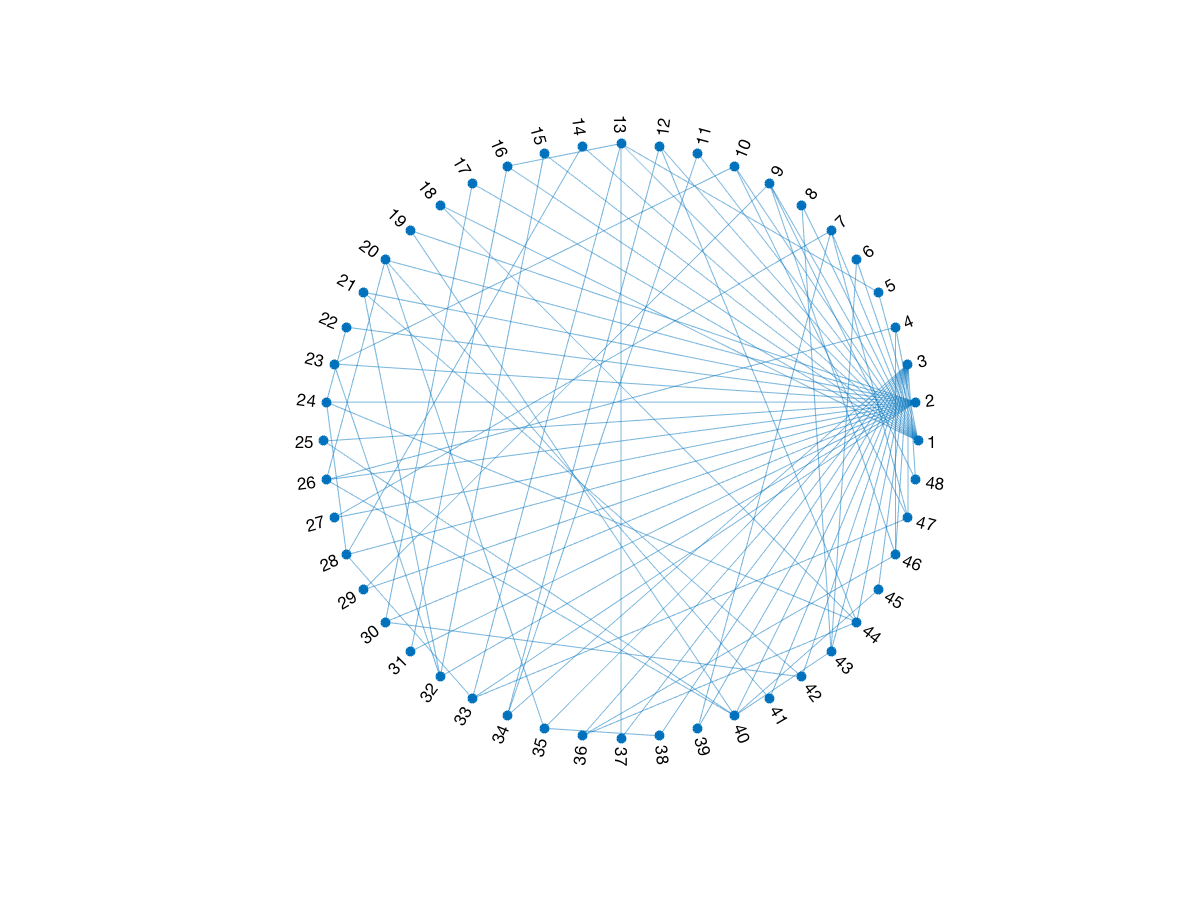
\includegraphics[width=6cm]{fig/disjoint_graph} 
  &   \includegraphics[width=3.5cm]{fig/disjoint_true}
   \\    (a) \textit{model 1} & (b)  structure of concentration matrix for \textit{model 1} \\
      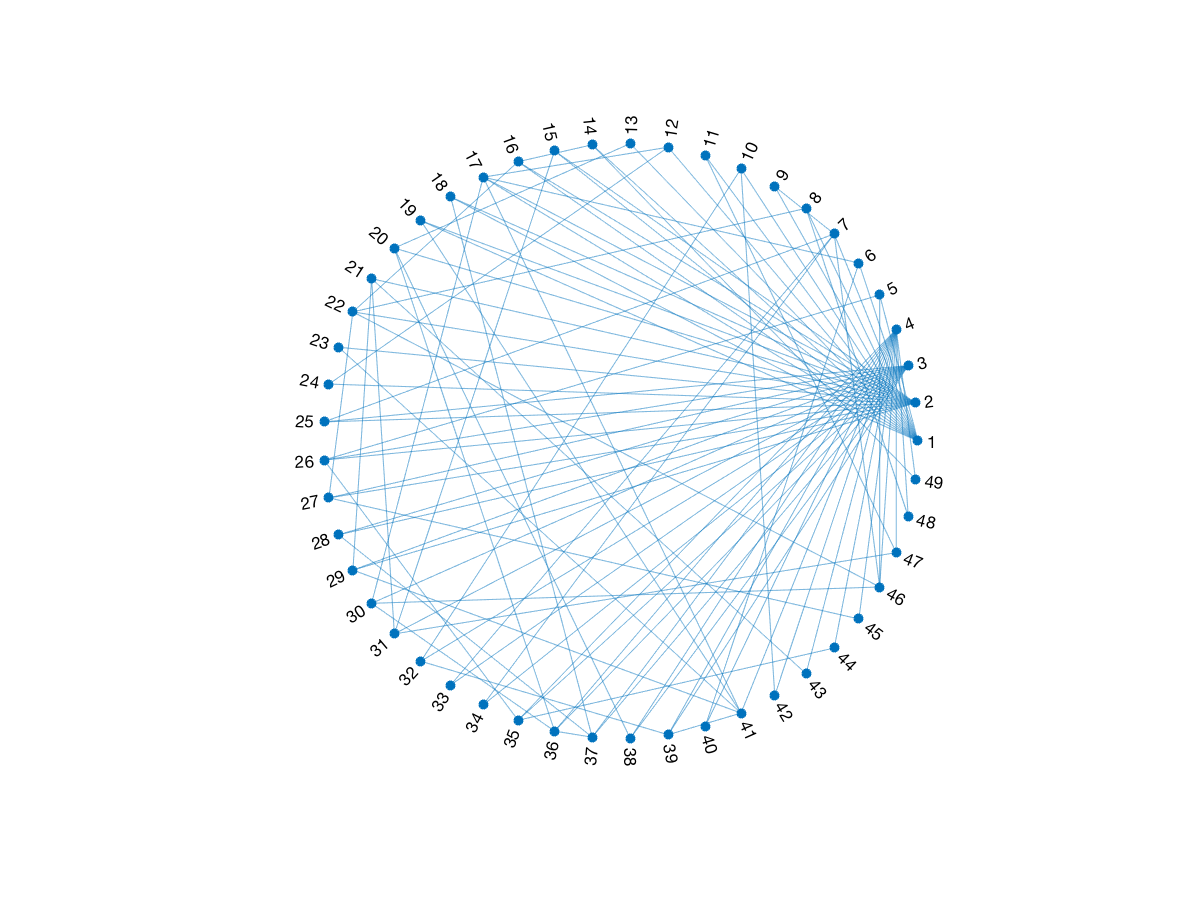
\includegraphics[width=6cm]{fig/over_graph} 
  &   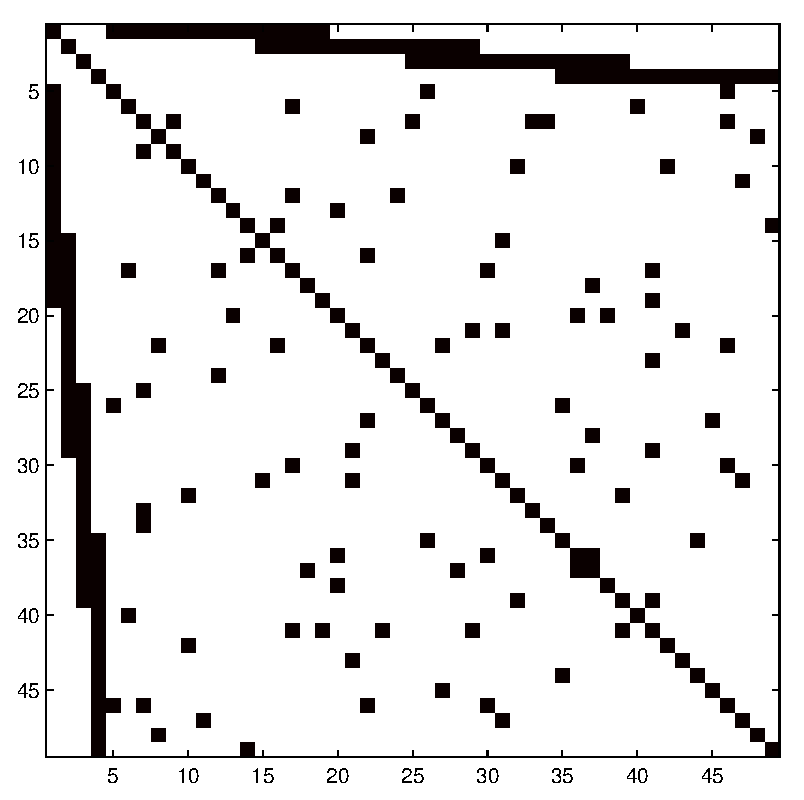
\includegraphics[width=3.5cm]{fig/overlap_true}
   \\    (c) \textit{model 2} & (d)  structure of concentration matrix for \textit{model 2} \\
      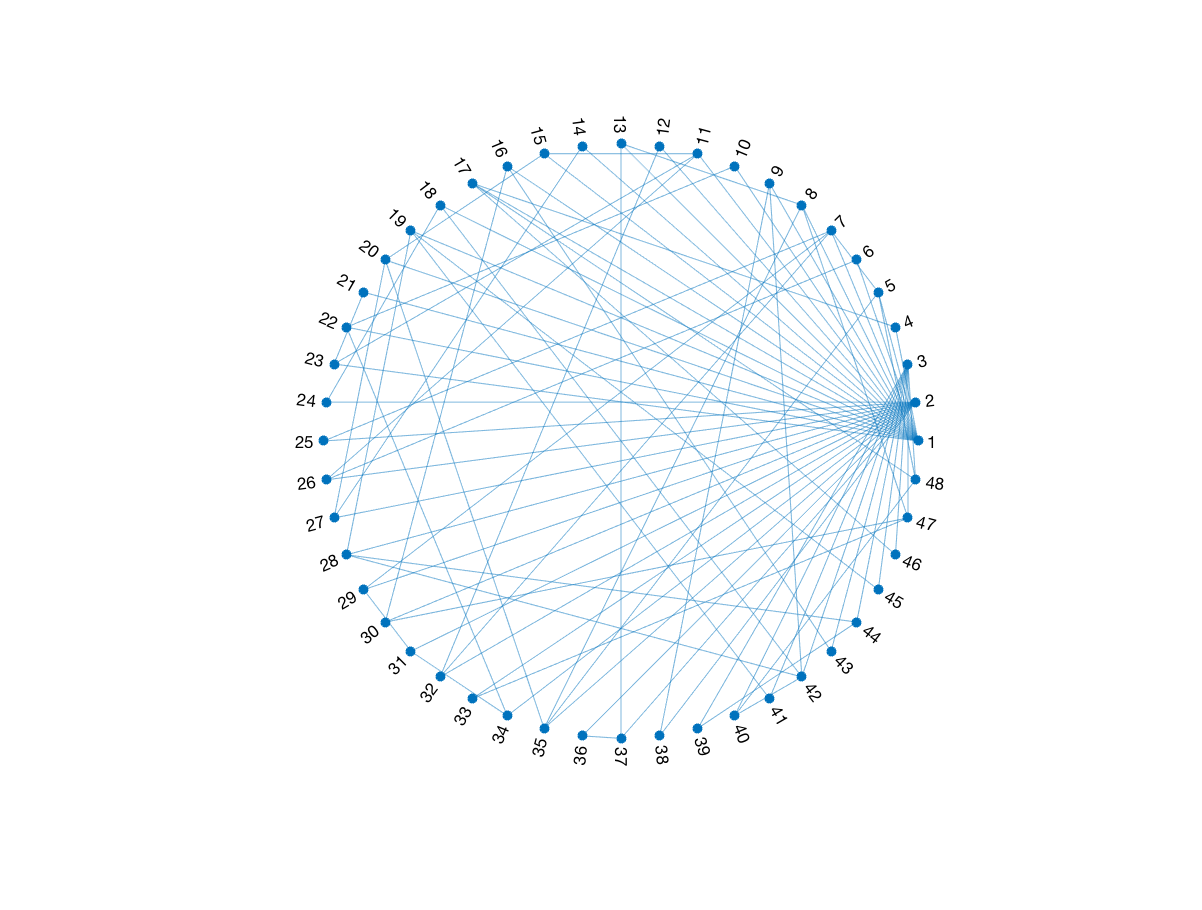
\includegraphics[width=6cm]{fig/diff_graph} 
  &   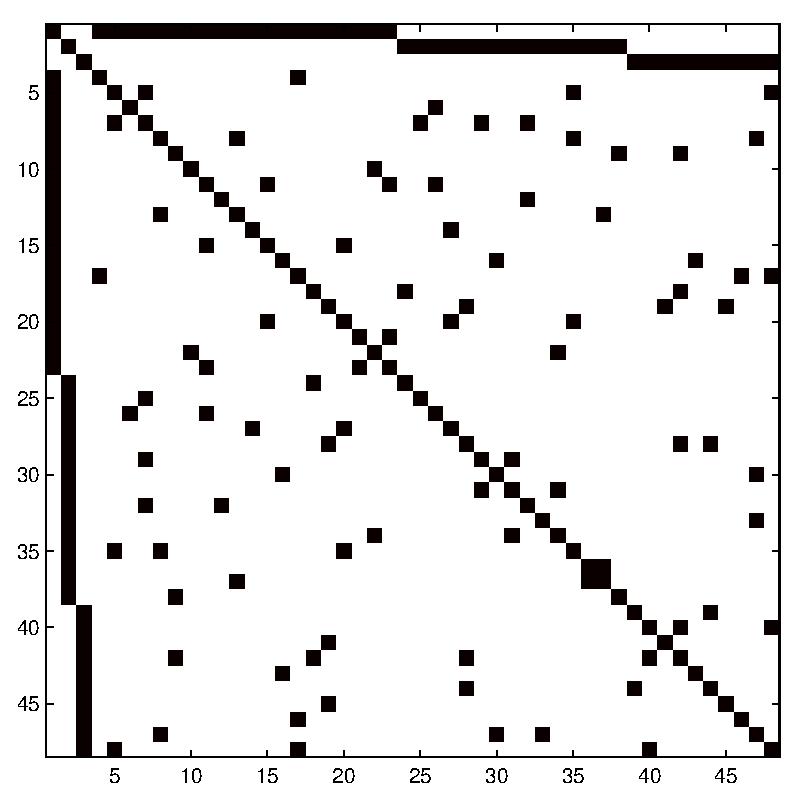
\includegraphics[width=3.5cm]{fig/diff_true}
   \\    (e) \textit{model 3} & (f)  structure of concentration matrix for \textit{model 3}
\end{tabular}
\caption{ Structures of graphical models for the synthetic experiments}
\end{figure}

\begin{figure}
\center
\begin{tabular}{cccc}
      \includegraphics[width=4cm]{fig/MILE_Som}
  &   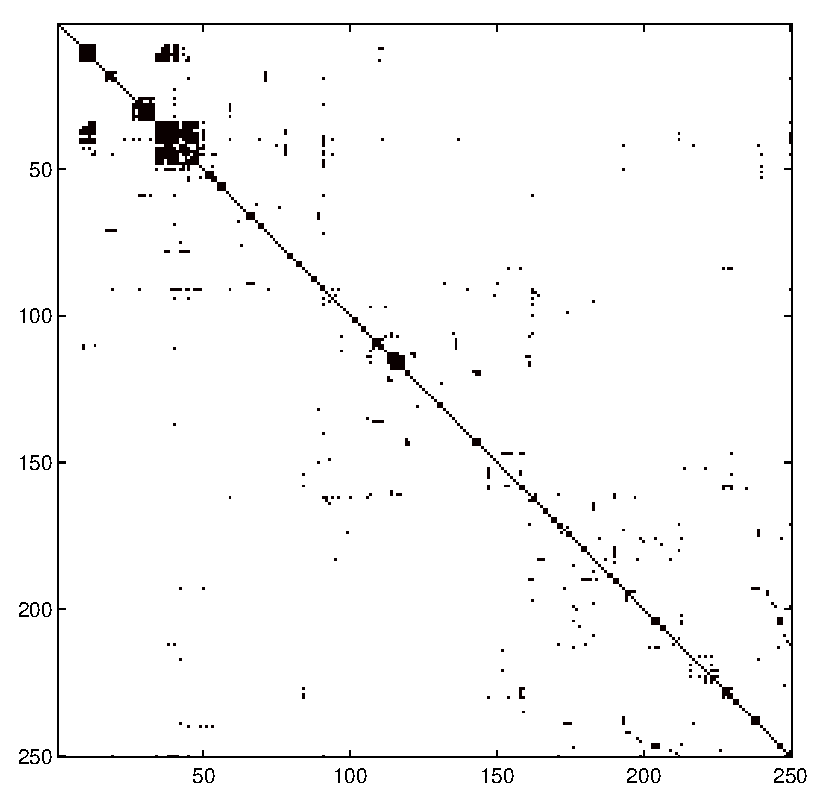
\includegraphics[height=3.8cm]{fig/MILE_Ssl_ordered}
   \\   (a)  $\hat{S}$ $\ell_1+\tr$  & (b) $\hat{S}$ ours 
\end{tabular}
\caption{Sparse component for our method (a) for maximum log-likelihood regularized by $\ell_1+\tr$ (b) }
\end{figure}


\section*{References}
\bibliographystyle{apalike}
\bibliography{lvggm}

\end{document}
